\documentclass[French,Hoar.tex]{subfiles}

\begin{document}

  \section{La logique de \h}
  %src https://www.cs.cmu.edu/~aldrich/courses/15-819O-13sp/resources/hoare-logic.pdf
  \subsection{Pr\e sentation}
    Le but de la \emph{Logique de \h} est de permettre un systeme formelle de raisonement 
    sur la justesse d'un programme \cite{Hoar:1}
    Plus concrettement comme chacun le sait il existe des systeme critique pour lequel l'incertitude
    n'est pas acceptable.
    Cette logique est baser sur les \textbf{\color{nred}{ triplet de \h}},
    ce triplet de la forme $\{P\} S \{Q\}$ est respectivment composer de :
    %TODO ajouter plus d'explication
    \begin{itemize}
      \item[\ding{227}] $P$ Une precondition
      \item[\ding{227}] $S$ Le programme
      \item[\ding{227}] $Q$ Une postcondition
    \end{itemize}
    Les precondition est postcondition sont deux assertion appartenant a la \href{http://zanotti.univ-tln.fr/MD/MD-Ensembles.html#pr%C3%A9dicats}{logique des predicats}.
    Un triplet de hoare est correct si la condition initial $P$ est verifier est $S$ executer ce qui implique que
    $Q$ est vrai.

    \emph{exemple:}
    \begin{center}
     $\{x = 5\} x := x\times 2 \{x > 0\}$ 
    \end{center}
    Ce triplet est clairement correct, en effet si $x=5$ est que $x$ est multplier par deux, $x$ est bien sur 
    superieur a 0.


  \subsection{M\e thode}
  Ce triplet est un outils essentielle car il permet grace a de nombreuse propriete (voir plus bas), de realiser des preuve rigoureuse de nos 
  algorithme. Il y a cependant un problème important et il s'agit de S, en effet dans le cas d'une boucle nous cherchons qu'elle que chose de complexe 
  a trouver un \emph{invariant de boucle} par exemple:
  \begin{lstlisting}[style=C]
  int somme(int n):
    int s = 0;
    for(int i=0;i<n+1;i++)
        s++;
    return s;
\end{lstlisting}
Ici l'invariant de boucle est $s=\sum_{k=0}^{i-1} k$

Maintenant qu'elle que propriete:

  \begin{mytheo}{Axiome de l'affectation}{Axiome de l'affectation}
    L'affectation est l'instruction x := E , associant à la variable x la valeur de l'expression E.
    $$
    \frac{}{\{P[E/x]\}\ x:=E \ \{P\} } 
    $$
  \end{mytheo}


  \begin{mytheo}{Règle de composition}{Règle de composition}
    La règle de composition s'applique pour les programmes $S$ et $T$ s'ils sont exécutés séquentiellement, où $S$ s'exécute avant $T$. Le programme issu de cette exécution est noté $S;T$.
    $$
 \frac {\{P\}\ S\ \{Q\}\ , \ \{Q\}\ T\ \{R\} } {\{P\}\ S;T\ \{R\}}
    $$
  \end{mytheo}


  \begin{mytheo}{Règle de la conditionnelle}{Règle de la conditionnelle}
La règle de la conditionnelle permet de combiner deux programmes dans un bloc $'si...fin\ si$', lorsque les conditions le permettent.
    \begin{align*}
 &\frac {\{P\}\ S\ \{Q\}\ , \ \{Q\}\ T\ \{R\} } {\{P\}\ S;T\ \{R\}}\\
 &\textbf{si}\ B\ \textbf{alors}\ S\ \textbf{sinon}\ T\ \textbf{fin\ si}\ \{Q\}\\
 \end{align*}

  \end{mytheo}
  Le reste des propriete peuvent etre retrouver \href{https://fr.wikipedia.org/wiki/Logique_de_Hoare#Axiome_de_l%27affectation}{ici}
  \subsection{Application}
  Maintenant cette logique de \h peut sembler interesante pour un mathematicien est sans doute stimulante pour
  l'infomaticien avide d'impressioner ces paire mais pourtant des application concrete, essentielle et r\e cente existe.

  Avant de parler de l'une de ces aplication concrete une definition :
   \begin{definition}
    Un language est dit \textbf{Type-Safe} si il ne permet pas les erreur de type.
  \end{definition}
  \begin{verbatim}
    exemple:
    a="Toulon" ;a++

    ~~~~~~~~~~~~~~~~~~~~~~~~~~~~~
    errors: you cannot add to an
    str, it has no sens...
    moron
  \end{verbatim}
  En generale il existe une connexion entre la \emph{Type-Safety} est les problème de m\e moire.
  Bien sur tout cela peut sembler eminament utile pour un programmes ou meme un language, mais certaine
  chose peuvent sembler plus essentielle que d'autre par exemple un \text{\color{nred}{OS}}.

  C'est ce que a essayer de faire des checheur de Microsoft et du M.I.T en creant un OS X86 type-safe.

  \begin{figure}[H]
    \centering
  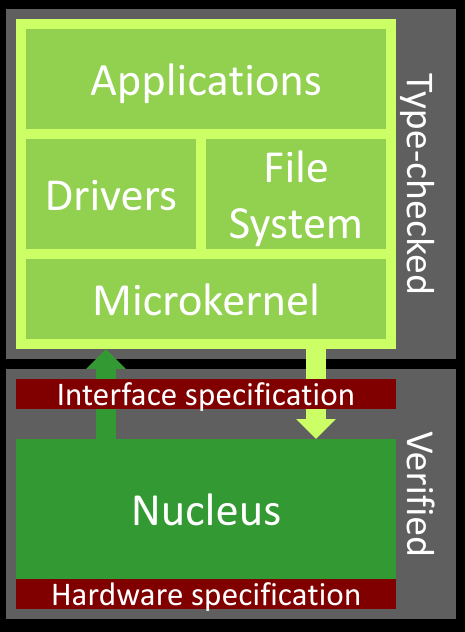
\includegraphics[scale=0.2]{./img/Verve.png}
  \caption{Diagrame de Verve}
  \label{fig:Verve}
\end{figure}

  Cette OS baser bien sur sur la logique de \h, a etait cree en utulisante \emph{Boogie} un outils en ligne
  permettent dans beaucoup de cas, pas touts, de verifier de maniere formelle la justesse d'un algorithme.
  Il ouvrent bien sur des perspective interesante pour le future.

\end{document}
